\chapter*{Anexo H: Tutoriales}

\label{AnexoHTutoriales}

\subsubsection{Primer Tutorial}

En el primer tutorial, se pretende familiarizar al jugador con la pantalla, demostrando que los planetas son navegables y que existen caminos que los conectan, permitiendo hacer clic entre ellos. En esta etapa, también se proporciona información sobre el diálogo y se presentan pistas visuales.


\begin{figure}[h]
	\centering
	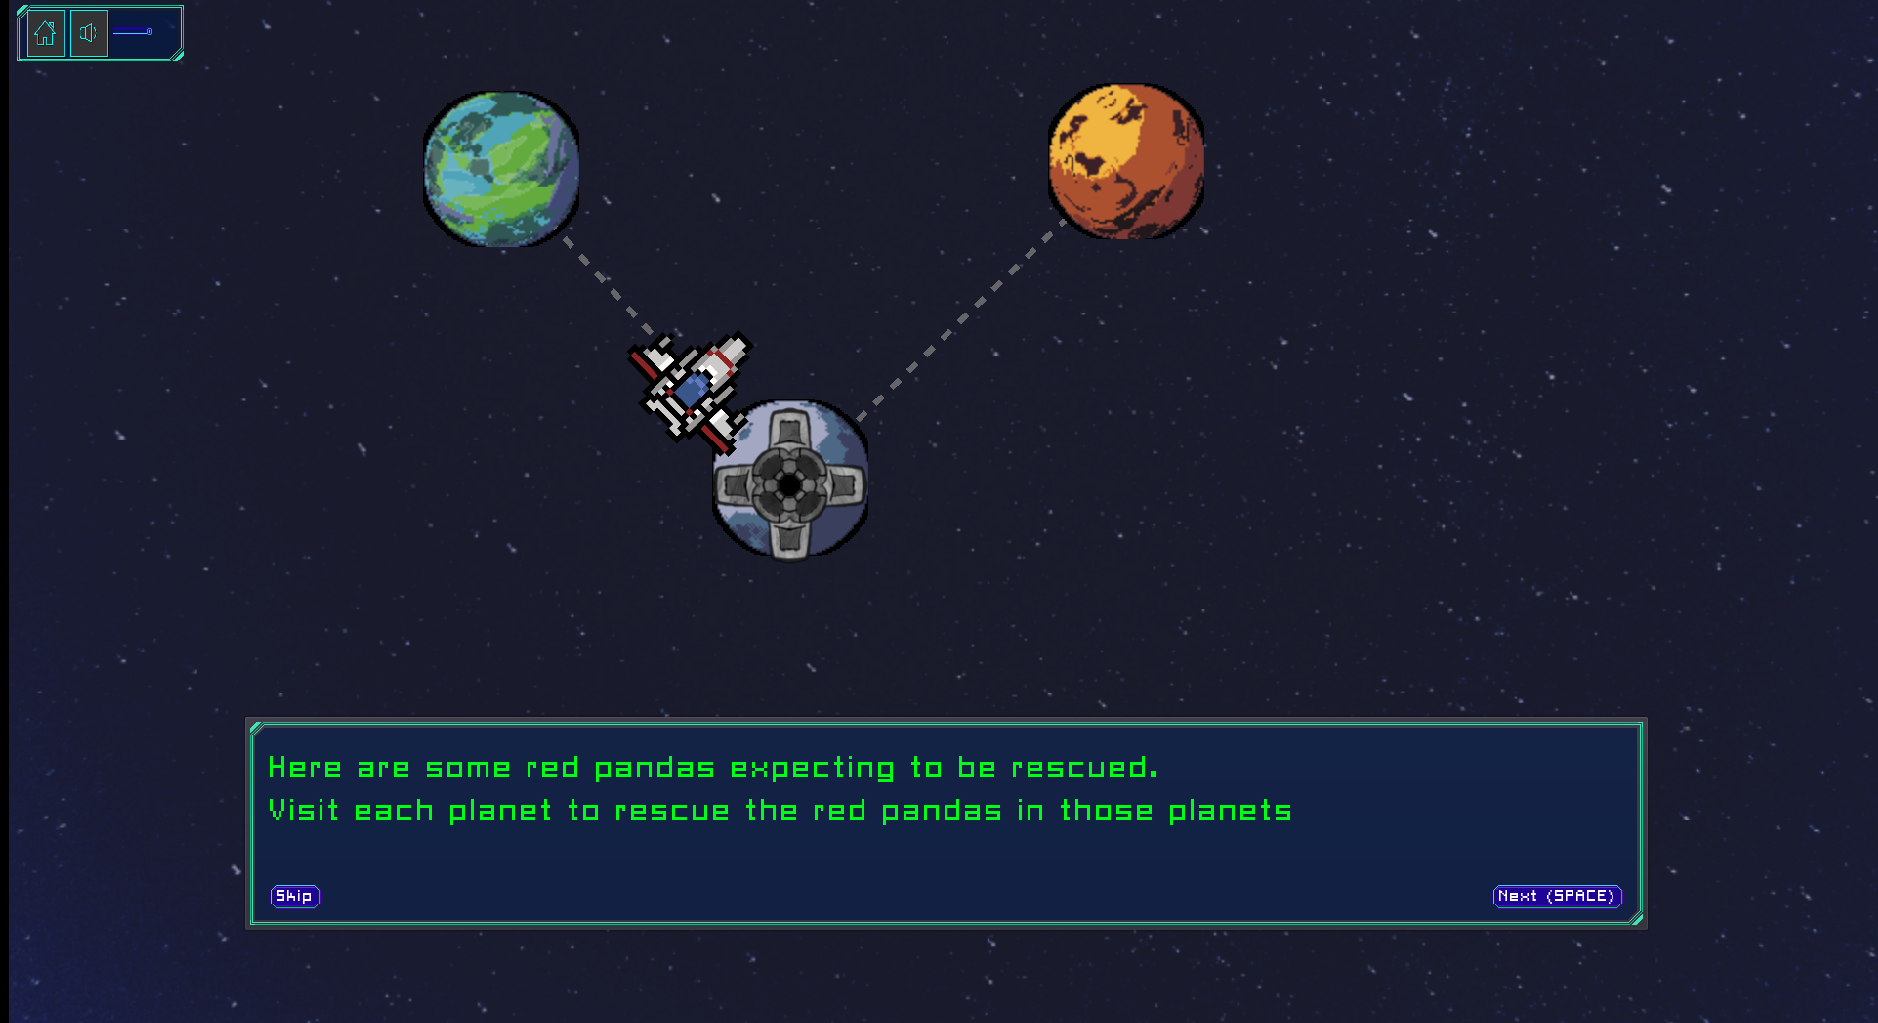
\includegraphics[scale=0.3]{imagenes/FirstTutorial.png}
	\caption{Primer tutorial. Se le indica al jugador a través de un diálogo que debe visitar cada planeta.}
	\label{FirstTutorial}
\end{figure}



\subsubsection{Segundo tutorial}

En el segundo tutorial, se presenta la mecánica de instrucciones e introduce el ciclo for y el if en las instrucciones, elementos que se utilizarán más adelante.

Al inicio del segundo tutorial, se le indica al jugador que debe seguir las instrucciones del algoritmo debido a que la exploración automatizada de los pandas rojos es costosa y el combustible se está agotando. Las primeras dos instrucciones solicitan al jugador que presione la tecla espacio para avanzar a la siguiente instrucción (ver figura \ref{SecondTutorial}).


\begin{figure}[h]
	\centering
	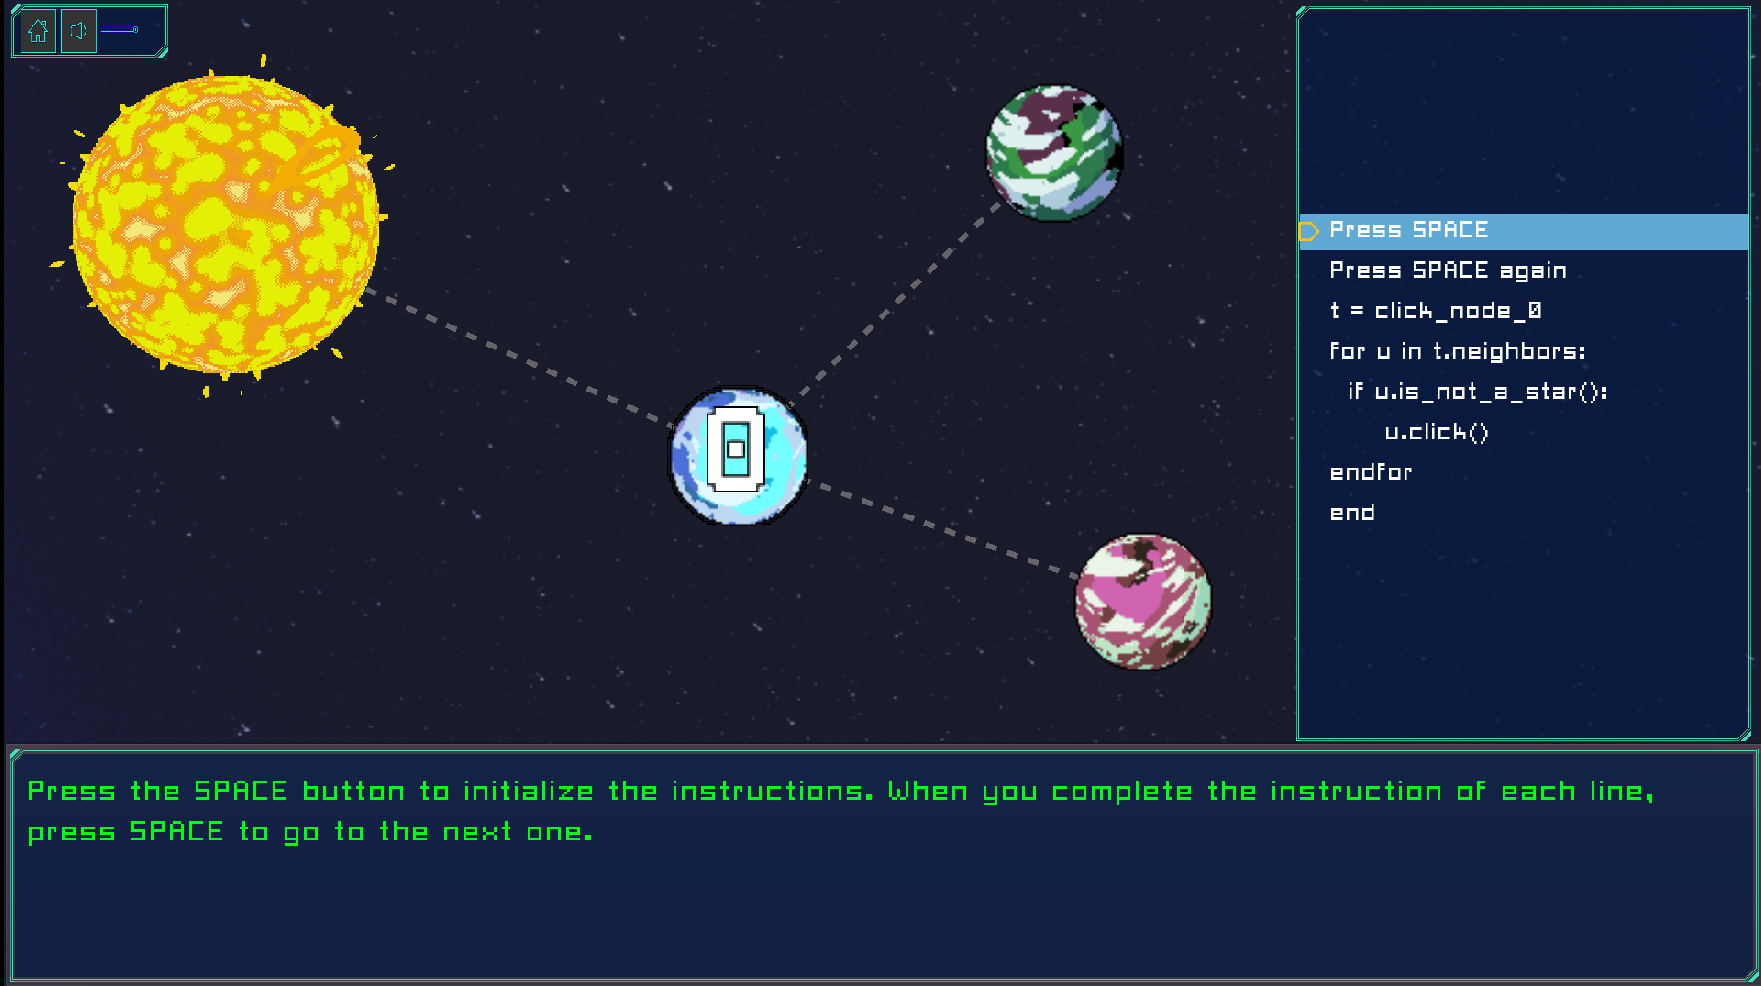
\includegraphics[scale=0.2]{imagenes/SecondTutorial.png}
	\caption{Segundo tutorial. Se le muestra un diálogo de entrada al jugador introduciéndole el nuevo concepto. Este es el primer momento en que se le muestran las instrucciones al jugador.}
	\label{SecondTutorial}
\end{figure}

Durante este segundo tutorial, se introduce la lógica de responder sí o no cuando aparece una instrucción con un if. El jugador debe dar la respuesta correcta para avanzar a la siguiente instrucción. Si responde incorrectamente, perderá y deberá reiniciar el nivel. En la figura \ref{SecondTutorialShowingIf}, se muestra la ventana que aparece al jugador al llegar a una instrucción con un if.

\begin{figure}[h]
	\centering
	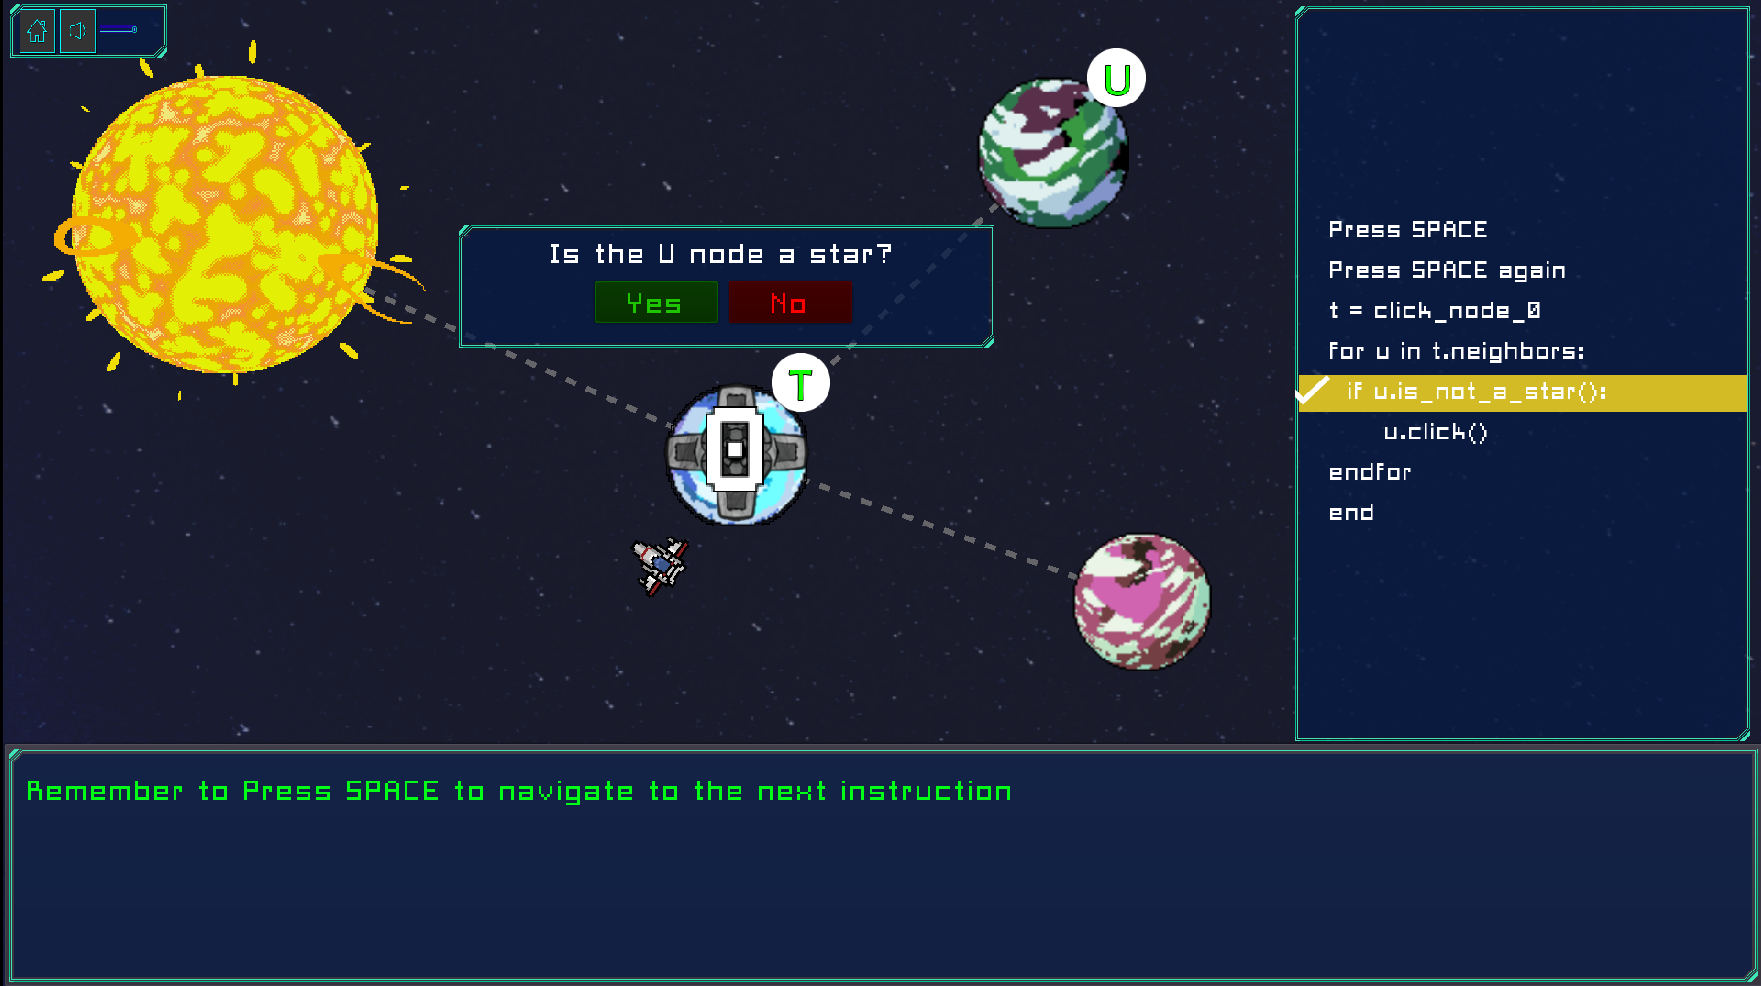
\includegraphics[scale=0.3]{imagenes/SecondTutorialShowingIf.png}
	\caption{Segundo tutorial. Ventana de if que le aparece al jugador al llegar a una instruccion con un if. El jugador debe responder sí o no correctamente para avanzar}
	\label{SecondTutorialShowingIf}
\end{figure}

\subsubsection{Tercer tutorial}

El tercer tutorial introduce al jugador el concepto de Pilas (Stacks) y Colas (Queues) como estructuras de datos para almacenar nodos y luego obtenerlos en órdenes distintos. Además, se le introduce al jugador sobre las variables creadas y la variable seleccionada, la cual se usa para señalar a qué objeto se le agregará el nodo que el usuario presione.

\begin{figure}[h]
	\centering
	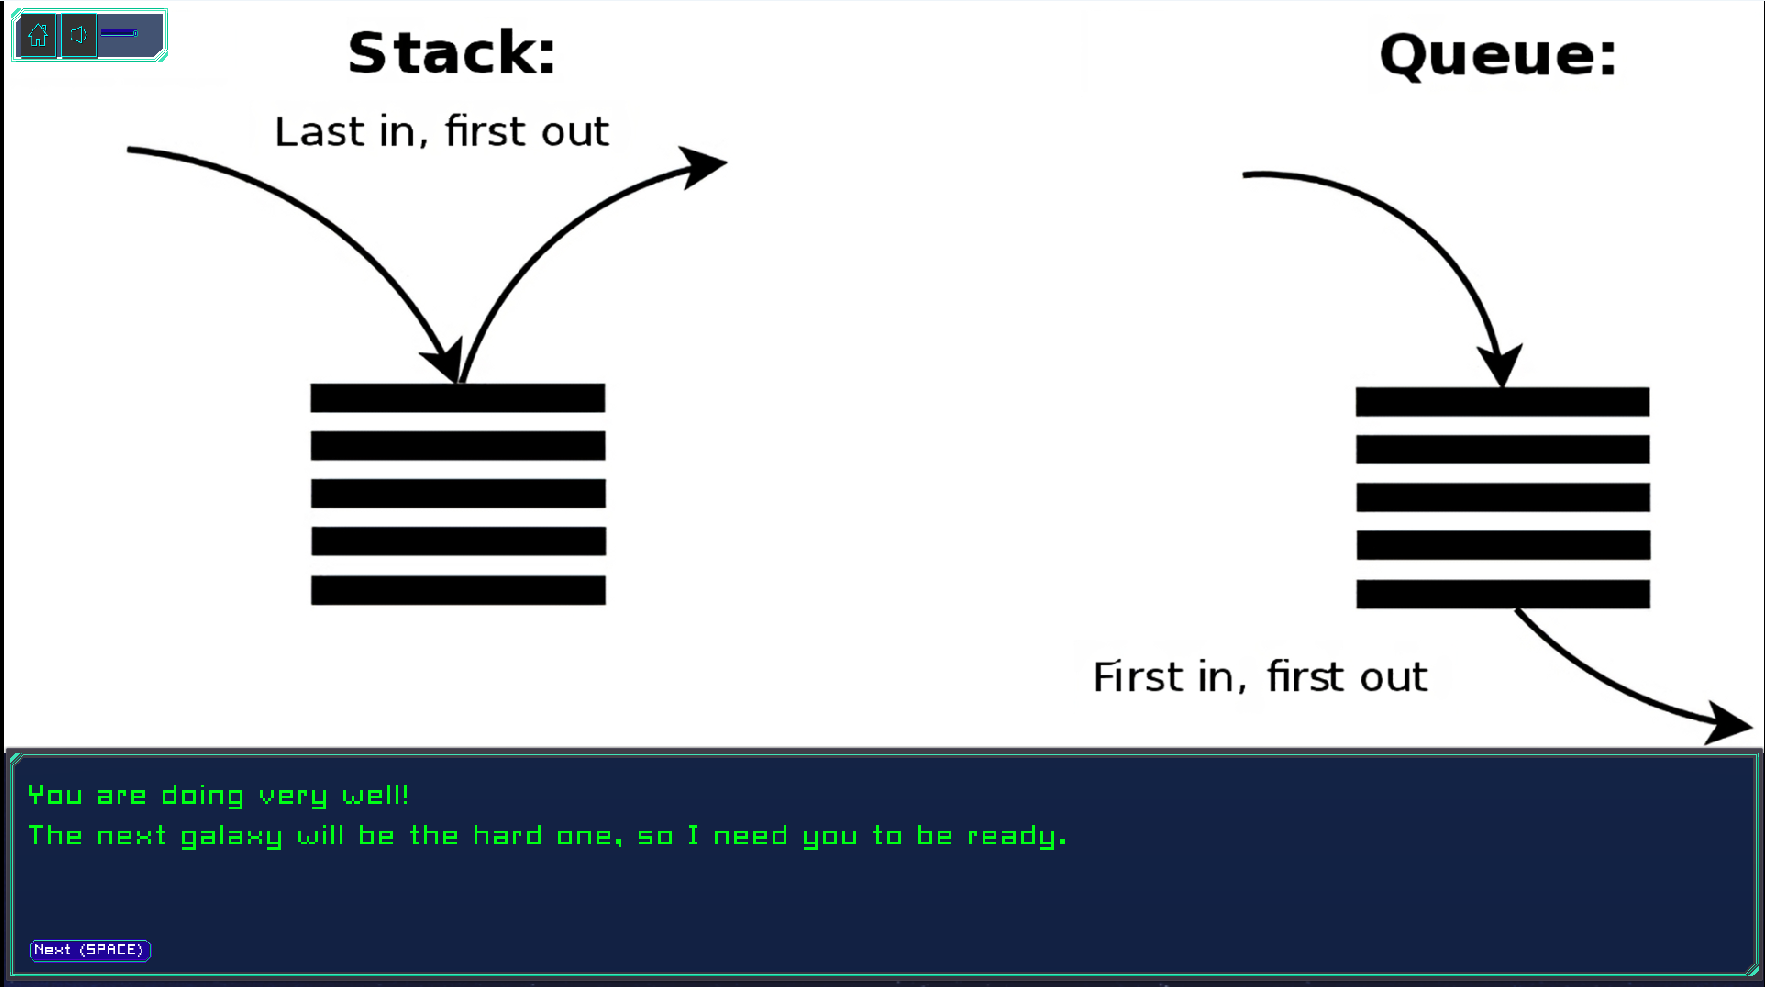
\includegraphics[scale=0.3]{imagenes/ThirdTutorialFirstDialogue.png}
	\caption{Tercer tutorial. Se le explica al usuario al inicio qué son las colas y stacks y cómo funcionan y en qué difieren.}
	\label{ThirdTutorialFirstDialogue}
\end{figure}


\begin{figure}[h]
	\centering
	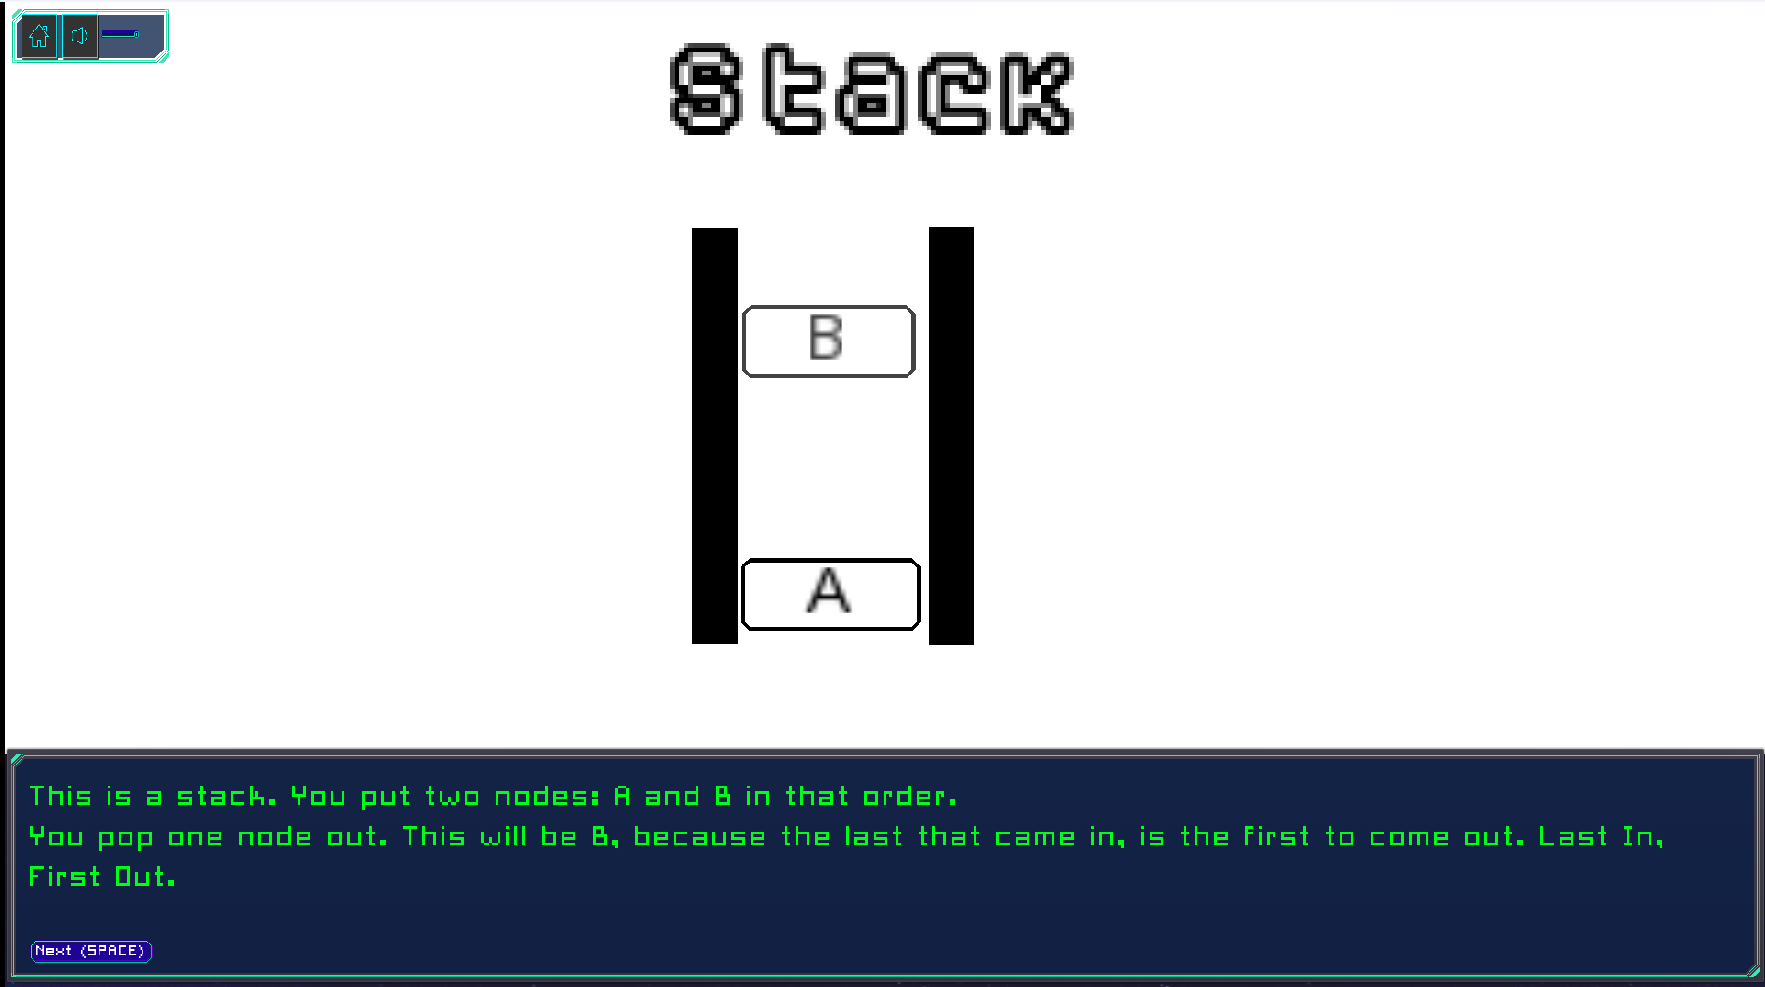
\includegraphics[scale=0.3]{imagenes/ThirdTutorialStackExplanation.png}
	\caption{Tercer tutorial. Mostrando al usuario cómo funciona un stack a través de animaciones.}
	\label{ThirdTutorialStackExplanation}
\end{figure}


El objetivo de las instrucciones en este tutorial es que el jugador aprenda la mecánica para agregar nodos a un stack o a una pila. Además, se refuerza la mecánica de las instrucciones y ejecutar cada acción paso por paso.


\begin{figure}[h]
	\centering
	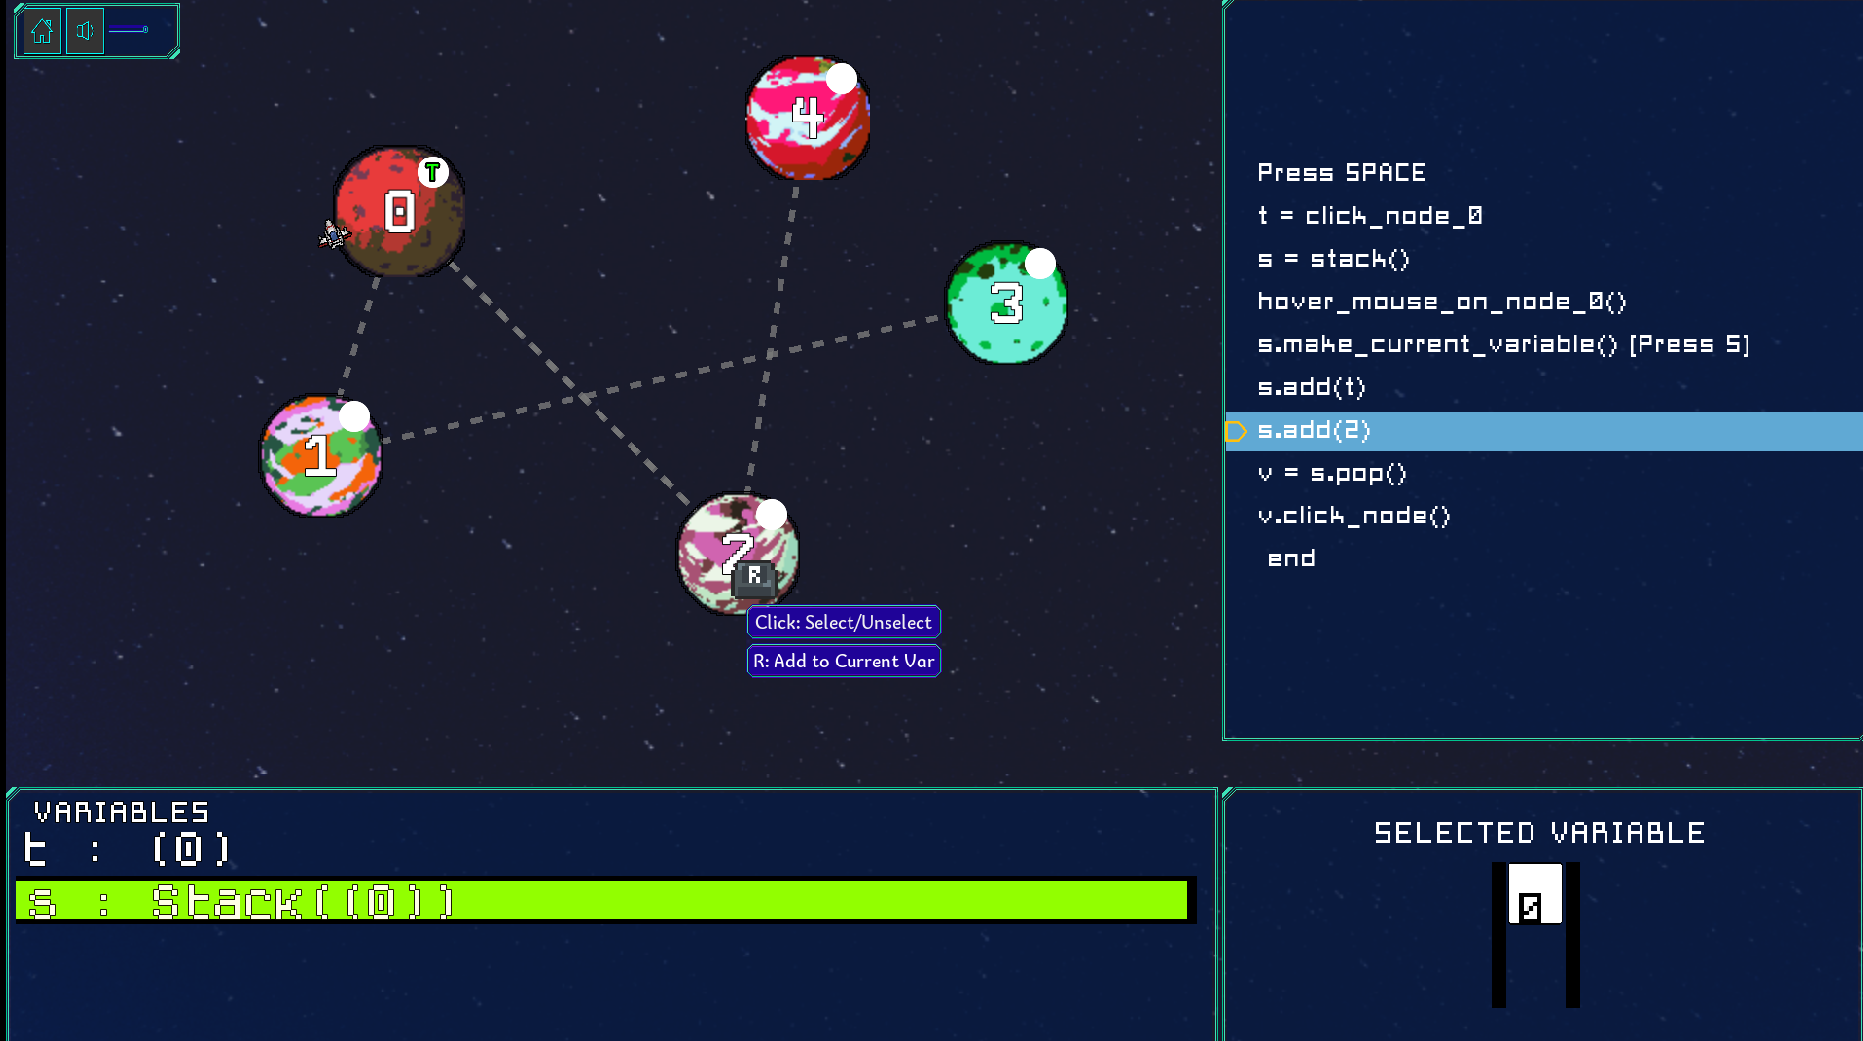
\includegraphics[scale=0.3]{imagenes/ThirdTutorialAddingNode.png}
	\caption{Tercer tutorial. El jugador debe presionar R sobre el planeta 2 para avanzar a la siguiente instrucción.}
	\label{ThirdTutorialAddingNodesToStacks}
\end{figure}
